\documentclass{IEEEtran}

\usepackage{hyperref}
\usepackage{graphicx}

\title{Hate speech detection - For Arabic Hate Speech 2022 Shared Task Competition}
\author{Prof Ensaf Hussein \\Kirollos Hany, Kirollos George, Malak Emad, \\ Shady Zekry, Seif Hesham, Fady Fayek}
\date{}

\graphicspath{{graphics/}}

\begin{document}
	
\maketitle

\begin{abstract}
	Hate speech and offensive language became a crucial problem nowadays due to large using of social media and internet by people from different gender, nationality, religion and other types of characteristics. In this paper we propose to make an automatically solution to this problem because it is very important for online safety, content moderation and solve racist problem. Most of models implemented to solve this problem were developed for English. So we introduce 2 Arabic nlp models. The first help to detect whether a tweet is offensive or not and we achieve over 79\%, 85\% and 82\% for precision, recall and f1-score for not offensive tweets and 83\%, 76\% and 79\% for precision, recall and f1-score for offensive tweets using logistic regression and marbert as feature extraction , the second model detect whether a tweet has hate speech or not and we achieve over 90\%, 91\% and 91\% for precision, recall and f1-score for not hate speech tweets and 91\%, 90\% and 91\% for precision, recall and f1-score for  hate speech tweets using logistic regression and marbert as feature extraction. Dataset used for training and testing models is tweets from Arabic Hate Speech 2022 shared task competition and we solve imbalanced in this dataset by using data augmentation.
\end{abstract}

\section{Introduction}
The increase in online hate speech is a major cultural threat, as it already resulted in crime against minorities, see e.g. (Williams et al. 2020). To tackle this issue, there has been a rising interest in hate speech detection to expose and regulate this phenomenon. Arabic hate speech detection has been a very challenging field among the hard ways we can get filtered data that are labeled and pre-classified. And how small data that you can find related to hate speech specifically for Arabic language.
Many resourceful and helpful models have been made available in the recent years by the community, towards the development of automatic hate speech detection for Arabic language, such as ARBERT and MARBERT which are Deep Bidirectional Transformers that are pretrained for Arabic language based on Google's BERT architecture. These models revolutionized the research on NLP and became resourceful in our feature-extraction phase. 
Another problem that is presented by the dataset is that it’s not balanced. The non-hate speech to hate speech ratio in the corpus is 9:1, our approach to solve this problem was to use data augmentation method, and a tool that helps us in that step is NLPAUG, we used it to solve the unbalancing in dataset by augmenting the sentences that are labeled as hate speech. That will result in a much larger count of how many rows feeded into the machine learning model labeled as hate speech, and that will help in the model learning phase.
The most popular approach to this problem is to use a deep-learning algorithm which does its own feature extraction, but in this case it’s not suitable because we need a huge dataset, and that is not the case in our Arabic dataset. Instead, we use multiple machine-learning approaches which are not greatly affected by the small size of the dataset. For feature extraction we use MARBERT model, then we feed the output to our two models (Logistic regression, Random Forest).


\section{Related Work}
Our goal in this task was to find the best approach to tackle the problem. First trying we have used tfidf technique, but the problem was that model was detecting words by its own meaning only without looking how it would be helpful for the context. Second method we moved into using MARbert after searching for a method that helps in understanding the whole paragraphs and give the meaning for each word. It is made by extracting every single word as a vector in vector space representing in our case tweets. Then the method we used MARbert is by extracting features for our Logistic Regression model or our Random Forest model. The most appealing results relatively appeared in Random Forest model with results: 79\%, 85\% and 82\% for precision, recall and f1-score for not offensive tweets and 83\%, 76\% and 79\% for precision, recall and f1-score for Logistic Regression, and for Random Forest 90\%, 91\% and 91\% for precision, recall and f1-score for not hate speech tweets and 91\%, 90\% and 91\% for precision, recall and f1-score. One of the challenges we have faced that data we used in training was heavily biased towards not-offensive hate speech tweets, so after a lot of researching we have used NLP Augmenter to generate new hate speech tweet to balance the data.


\section{Methods and Materials}
The problem we have face on finding the problem of unbalanced data set. We have used data visualization methods to find where the issue is in first place. The graphs down below shows how the model is biased.

\begin{figure}[htbp]
	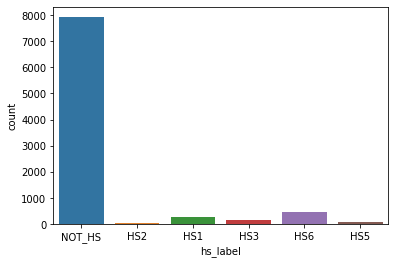
\includegraphics[width=\columnwidth, height=0.30\paperwidth]{02.png}
\end{figure}

Then after applying the NLP aug, the data set was balanced in a reasonable manner.

\begin{figure}[htbp]
	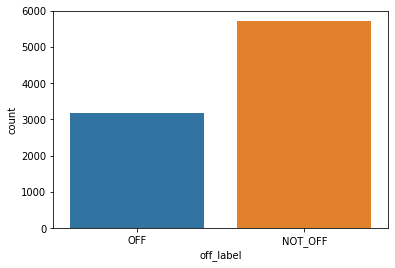
\includegraphics[width=\columnwidth, height=0.22\paperheight]{01.png}
\end{figure}

The data set we have used we split it into 2 parts. First part is testing data which is 70\%, and testing data which represents 30\%. Worth mentioning that the data set is from the \href{https://sites.google.com/view/arabichate2022/home}{competition}.

\section{Conclusion}
We present an approach to detect Hate speech texting detection based on natural language processing.our approach can be applied to detecting hate speech dialogue which is composed of pure text.
The challenge was to find a way to detect hate speech in the Arabic language, as the data set imbalanced, and we overcame that by using the data augmentation method and NLPAUG tool helped us.
Using logistic regression and marbert as feature extraction we got 91\%, 90\% and 91\% for precision, recall and f1-score for hate speech tweets.
Furthermore, we aim to develop a more balanced dataset and execute the algorithm in a real environment. The results will indicate if any new algorithms might be necessary to improve
detection.



%
% Starting bibliography
%

\bibliographystyle{IEEEtran}
\bibliography{./citations.bib}

\end{document}
